% Derleme: XeLaTeX (Overleaf: Menu -> Compiler -> XeLaTeX)
% Sekiller ../results/figures klasorunden okunur.
\documentclass[11pt,a4paper]{article}
\usepackage{amsmath,amssymb}
\usepackage[no-math]{fontspec}
\setmainfont{TeX Gyre Termes}
\usepackage{polyglossia}
\setmainlanguage{turkish}
\usepackage[margin=2.1cm]{geometry}
\usepackage{graphicx,booktabs,multirow,float,microtype,xcolor,enumitem,caption,titlesec}
\usepackage[nocompress]{cite}
\usepackage[hidelinks]{hyperref}
\graphicspath{{../results/figures/}}
\captionsetup{font=small,labelfont=bf,labelsep=period}
\setlist{itemsep=2pt,topsep=4pt}
\titleformat{\section}{\large\bfseries}{\thesection.}{0.5em}{}
\titleformat{\subsection}{\normalsize\bfseries}{\thesubsection.}{0.5em}{}
\setlength{\parskip}{3pt}
\setlength{\emergencystretch}{3em}
\renewcommand{\arraystretch}{1.12}
\newcommand{\nrmse}{nRMSE}

\begin{document}

\begin{center}
{\LARGE\bfseries Güneş Enerjisi Santrallerinde ANFIS Tabanlı Güç Tahmini:\\[2pt]
Yeniden Gerçekleştirme ve Sensör Gürültüsüne Dayanıklı Bir Genişletme}\\[10pt]
{\large Emre Açıl}\\[2pt]
Öğrenci No: 1306220081 \quad·\quad Bilgisayar Mühendisliği, İstanbul Üniversitesi-Cerrahpaşa\\
Bulanık Mantık Dersi — Dönem Projesi Teknik Raporu\\
Kod ve veri: \url{https://github.com/Aclmr/fuzzy-logic-project}
\end{center}

\begin{abstract}
\noindent Bu çalışmada Salameh vd.~\cite{salameh2025} tarafından önerilen, dört çevresel ölçümden (güneş ışınımı, ortam sıcaklığı, modül sıcaklığı, rüzgâr hızı) şebekeye bağlı bir fotovoltaik (PV) sistemin DC gücünü, gerilimini ve akımını tahmin eden ANFIS modeli yeniden gerçekleştirilmiştir. Referans çalışmanın verisi kamuya açık olmadığından aynı dört girdiyi ve üç çıktıyı ölçen açık lisanslı NIST Ground Array verisi \cite{nist} kullanılmış; ANFIS herhangi bir hazır kütüphane kullanılmadan NumPy ile sıfırdan kodlanmıştır. Makaledeki iki temel deney tekrarlanmış ve ana bulgu doğrulanmıştır: ANFIS, güç tahmininde doğrusal regresyon, karar ağacı, SVM ve rastgele ormana göre en düşük test hatasını vermiştir (test $R^2=0{,}9952$, normalize RMSE \%4,39; 10 farklı bölmenin 10'unda birinci). Özgün katkı olarak (i) kural tabanı karmaşıklığı, (ii) kronolojik bölmede zamansal genelleme ve (iii) makalenin kendi sensör hassasiyetleri düzeyinde girdi gürültüsüne dayanıklılık incelenmiştir. ANFIS'in kronolojik bölmede doğruluğunu koruduğu, ancak gerçekçi sensör gürültüsünde SVM ve rastgele ormanın gerisine düştüğü gösterilmiştir. Bu zayıflığa karşı önerilen \emph{Robust-ANFIS} (gürültü enjeksiyonlu eğitim), model yapısını ve parametre sayısını değiştirmeden gerçekçi gürültüde hatayı \%16, iki kat gürültüde \%29 azaltmış; bunun bedeli temiz veride hatanın \%4,32'den \%4,89'a çıkması olmuştur.
\end{abstract}

% =====================================================================
\section{Introduction — Giriş}

Fotovoltaik (PV) sistemlerin ürettiği güç, ışınım ve sıcaklık gibi çevresel değişkenlere doğrusal olmayan biçimde bağlıdır. Şebeke işletmecisi açısından bu değişkenlik, üretimin doğru tahmin edilmesini; sistem sahibi açısından ise ölçülen üretimin \emph{beklenen} üretimle karşılaştırılarak arızaların erken fark edilmesini gerekli kılar \cite{salameh2025,gaboitaolelwe2023}. Fiziksel modeller (ör. sıcaklık katsayılı MPP denklemleri) panel parametrelerini ve kayıp mekanizmalarını ayrıntılı bilmeyi gerektirirken, salt veri güdümlü yöntemler (derin ağlar, topluluk modelleri) çoğu zaman yorumlanamaz \cite{gaboitaolelwe2023}. Bulanık mantık bu iki uç arasında bir köprü kurar: “ışınım yüksek \emph{ve} panel sıcaksa güç şöyledir” biçimindeki dilsel kurallarla belirsizliği temsil eder; ANFIS ise bu kuralların parametrelerini veriden öğrenir \cite{jang1993}.

Referans makale \cite{salameh2025}, Sharjah'taki (BAE) 2,88~kW'lık bir çatı sistemi için birinci dereceden Sugeno tipi bir ANFIS geliştirmiş; DC güç için test $R^2=0{,}9967$ raporlamış ve ANFIS'in dört klasik makine öğrenmesi modelinden daha iyi genellediğini ileri sürmüştür. Ancak makale yalnızca temiz veri ve rastgele bölme ile değerlendirme yapmakta, kural sayısını gerekçelendirmemekte ve verisini paylaşmamaktadır.

Bu projenin amaçları şunlardır:
\begin{enumerate}[label=(\arabic*)]
\item Referans yöntemi açık bir veri seti üzerinde, kütüphane kullanmadan yeniden gerçekleştirmek ve makaledeki Tablo~4 ile Tablo~5 deneylerini tekrarlamak;
\item Makalenin açık bıraktığı üç soruyu kontrollü deneylerle yanıtlamak: kaç kural gerekir, model gelecekteki veride çalışır mı, gerçekçi sensör hatasında ne olur;
\item Tespit edilen zayıflığa karşı yapıyı değiştirmeyen bir iyileştirme (Robust-ANFIS) önermek ve tüm modellerle adil biçimde karşılaştırmak.
\end{enumerate}

% =====================================================================
\section{Related Work — İlgili Çalışmalar}

PV güç tahmini literatüründe son yıllarda derin öğrenme ve hibrit modeller öne çıkmaktadır. Xiang vd.~\cite{xiang2024} TCN, ECANet ve GRU katmanlarını birleştirerek kısa dönem tahminde $R^2=\%99{,}72$ bildirmiştir. Fan vd.~\cite{fan2024} CNN-LSTM-dikkat mimarisinin hiperparametrelerini Crested Porcupine Optimizer ile ayarlamış; Ibrahim vd.~\cite{ibrahim2024} CNN ve LSTM otokodlayıcı hibritinin LSTM ve GRU'ya göre hatayı \%5–25 azalttığını ve eğitim süresini \%70 kısalttığını göstermiştir. Ait Mansour vd.~\cite{aitmansour2024} Bi-LSTM, GRU ve 1D-CNN modellerini karşılaştırarak gündüz verisinde $R^2=\%96{,}9$–$97{,}2$ elde etmiştir. Bashir vd.~\cite{bashir2024} ise referans makalenin de üzerinde çalıştığı Sharjah sisteminin verisiyle CNN-XGBoost hibritinde $R^2=\%99{,}62$ raporlamıştır. Gaboitaolelwe vd.~\cite{gaboitaolelwe2023} makine öğrenmesi tabanlı PV tahmin çalışmalarını derleyerek, sonuçların veri setine ve değerlendirme protokolüne güçlü biçimde bağlı olduğuna dikkat çekmiştir.

Bulanık ve nöro-bulanık yaklaşımlar tarafında Guerra vd.~\cite{guerra2024} ANFIS'in PV sistemlerindeki kullanımını (MPPT, modelleme, tahmin) kapsamlı biçimde derlemiştir. Perveen vd.~\cite{perveen2019} ANFIS tabanlı güneş enerjisi tahmin modelinin farklı gökyüzü koşullarında SVM, ileri beslemeli sinir ağı ve klasik bulanık modelden daha iyi sonuç verdiğini; Bouachrine vd.~\cite{bouachrine2023} ANFIS'in dört farklı PV teknolojisinde açık devre ve maksimum güç gerilimini analitik modelden daha doğru hesapladığını; Ramadan vd.~\cite{ramadan2022} ise ANFIS ile PV sistemlerin dinamik modelinin kurulabildiğini göstermiştir. Ren ve Zhou~\cite{ren2024} Takagi–Sugeno modeliyle PV gücünü belirsizlik bilgisiyle birlikte tahmin etmiştir. Massidda vd.~\cite{massidda2024} gün öncesi olasılıksal tahminde doğruluğu etkileyen faktörleri incelemiştir.

\begin{table}[H]
\centering\small
\caption{Seçilmiş ilgili çalışmaların karşılaştırması (değerler ilgili çalışmalarda raporlandığı gibidir).}
\label{tab:related}
\begin{tabular}{@{}llll@{}}
\toprule
Çalışma & Yöntem & Girdi / veri & Raporlanan sonuç \\
\midrule
Xiang vd.~\cite{xiang2024} & TCN-ECANet-GRU & Tarihsel güç + hava & $R^2=\%99{,}72$ \\
Bashir vd.~\cite{bashir2024} & CNN-XGBoost & Sharjah PV sistemi & $R^2=\%99{,}62$ \\
Ait Mansour vd.~\cite{aitmansour2024} & Bi-LSTM / GRU / 1D-CNN & a-Si şebeke sistemi & $R^2=\%96{,}9$–$97{,}2$ \\
Ibrahim vd.~\cite{ibrahim2024} & CNN + LSTM-AE & İngiltere güneş çiftlikleri & Hata \%5–25 düşük \\
Perveen vd.~\cite{perveen2019} & ANFIS & Meteorolojik değişkenler & SVM, FFNN, FL'den iyi \\
Salameh vd.~\cite{salameh2025} & ANFIS (SC, 4 kural) & 4 çevresel girdi, 601 örnek & Güç $R^2=0{,}9967$ \\
\textbf{Bu çalışma} & ANFIS + Robust-ANFIS & NIST, 4 girdi, 1555 örnek & Güç $R^2=0{,}9952$ \\
\bottomrule
\end{tabular}
\end{table}

Bu çalışmaların ortak eksikliği, modellerin genellikle temiz ve rastgele bölünmüş veride değerlendirilmesidir; girdilerdeki ölçüm hatasına duyarlılık nadiren raporlanır. Gürültü enjeksiyonuyla eğitimin modeli girdi bozulmalarına karşı düzenlileştirdiği bilinmektedir \cite{bishop1995}; bu çalışma bu fikri nöro-bulanık bir PV modeline, makalenin kendi sensör hassasiyetlerini kullanarak uygulamaktadır.

% =====================================================================
\section{Theoretical Background — Teorik Altyapı}

\subsection{Bulanık kümeler, üyelik fonksiyonları ve dilsel değişkenler}
Klasik kümede bir eleman ya kümeye aittir ya da değildir. Zadeh'in bulanık kümesinde~\cite{zadeh1965} $x$ elemanının $A$ kümesine aitlik derecesi $\mu_A(x)\in[0,1]$ üyelik fonksiyonu ile verilir. Örneğin 650~W/m²'lik bir ışınım “orta” kümesine 0,6, “yüksek” kümesine 0,4 derecesiyle ait olabilir. “Işınım”, değerleri “düşük, orta, yüksek” gibi bulanık kümeler olan bir \emph{dilsel değişkendir}. Bu çalışmada, referans makaledeki gibi Gauss üyelik fonksiyonu kullanılmıştır:
\begin{equation}
\mu(x)=\exp\!\left(-\frac{(x-c)^2}{2\sigma^2}\right),
\label{eq:gauss}
\end{equation}
burada $c$ merkez, $\sigma$ genişliktir. Gauss fonksiyonu türevlenebilir olduğundan gradyan tabanlı öğrenmeye uygundur.

\subsection{Bulanıklaştırma, kural tabanı ve çıkarım}
Bulanıklaştırma, kesin bir girdinin her bulanık kümeye üyelik derecesinin hesaplanmasıdır. Kural tabanı “EĞER $x_1$ $A_1$ VE $x_2$ $A_2$ İSE $y$ \ldots” biçiminde kurallardan oluşur. VE işlemi bir T-norm ile yapılır; bu çalışmada çarpım kullanılmıştır. Bir kuralın \emph{ateşleme gücü} $w_j$, öncül kısmındaki üyelik derecelerinin çarpımıdır.

\subsection{Mamdani ve Sugeno çıkarımı, durulaştırma}
Mamdani modelinde~\cite{mamdani1975} kural sonucu da bir bulanık kümedir (“\ldots İSE güç YÜKSEK”); kural çıktıları birleştirilir ve kesin değer genellikle ağırlık merkezi (centroid) ile durulaştırılarak elde edilir. Takagi–Sugeno–Kang (TSK) modelinde~\cite{takagi1985} ise kural sonucu girdilerin bir fonksiyonudur. Birinci dereceden Sugeno modelinde
\begin{equation}
f_j = p_j x_1 + q_j x_2 + r_j x_3 + s_j x_4 + t_j
\label{eq:sugeno}
\end{equation}
olup çıktı, kural çıktılarının ateşleme güçleriyle ağırlıklı ortalamasıdır (\emph{wtaver}). Bu durulaştırma, centroid integraline gerek duymadığı için hızlıdır ve türevlenebilirdir.

\subsection{ANFIS mimarisi ve hibrit öğrenme}
ANFIS~\cite{jang1993}, Sugeno tipi bir bulanık çıkarım sistemini beş katmanlı bir ağ olarak ifade eder. $R$ kural ve $n=4$ girdi için:
\begin{align}
\text{K1 (bulanıklaştırma):}\quad & \mu_{ji}(x_i)=\exp\!\big(-(x_i-c_{ji})^2/2\sigma_{ji}^2\big)\\
\text{K2 (ateşleme gücü):}\quad & w_j=\textstyle\prod_{i=1}^{4}\mu_{ji}(x_i)\\
\text{K3 (normalizasyon):}\quad & \bar w_j = w_j\big/\textstyle\sum_{k=1}^{R} w_k\\
\text{K4 (kural çıktısı):}\quad & \bar w_j f_j,\qquad f_j \text{ Denklem~(\ref{eq:sugeno})}\\
\text{K5 (toplam çıktı):}\quad & \hat y=\textstyle\sum_{j=1}^{R}\bar w_j f_j
\end{align}
Öncül parametreler $\{c_{ji},\sigma_{ji}\}$ doğrusal olmayan, sonuç parametreleri $\{p_j,\ldots,t_j\}$ ise çıktıda doğrusaldır. Jang'ın \emph{hibrit öğrenme} kuralı bu yapıdan yararlanır: ileri geçişte öncüller sabitken sonuç parametreleri en küçük kareler (LSE) ile tek adımda en iyi değerine getirilir; geri geçişte hata öncül parametrelere geri yayılarak gradyan inişi uygulanır.

\subsection{Kural tabanının oluşturulması: grid partition ve subtractive clustering}
\emph{Grid partition}, her girdiye $m$ üyelik fonksiyonu atar ve tüm kombinasyonları kural yapar; $n$ girdide $m^n$ kural oluşur (4 girdi, 3 MF $\Rightarrow$ 81 kural). Bu “boyut laneti” parametre sayısını hızla artırır. \emph{Subtractive clustering}~\cite{chiu1994} ise her veri noktasının çevresindeki nokta yoğunluğunu bir “potansiyel” olarak hesaplar, en yüksek potansiyelli noktayı küme merkezi seçer, onun çevresinin potansiyelini düşürür ve işlemi tekrarlar. Her küme bir kural olur; böylece kural sayısı verinin yapısına göre belirlenir ve küme yarıçapı $r_a$ ile kontrol edilir. Referans makale bu yöntemi kullanmıştır~\cite{salameh2025}.

% =====================================================================
\section{Original Method — Referans Yöntem}

\subsection{Sistem, veri ve model}
Referans çalışmada~\cite{salameh2025} Sharjah Üniversitesi çatısındaki 9 adet 320~W polikristal panelden oluşan 2,88~kW'lık şebekeye bağlı sistem kullanılmıştır. Sensörler: monokristal referans hücreli ışınım sensörü (±\%5), anemometre (±\%5) ve PT-1000 sıcaklık sensörleri (±0,8~°C). Haziran–Eylül döneminde toplanan 601 örneğin 410'u eğitim, 191'i test için kullanılmıştır. Girdiler ışınım, ortam sıcaklığı, modül sıcaklığı ve rüzgâr hızıdır; DC güç, gerilim ve akım için üç ayrı ANFIS kurulmuştur. Makalenin Tablo~1'ine göre model ayarları şunlardır: birinci dereceden (doğrusal) Sugeno çıktı, subtractive clustering ile oluşturulmuş 4 kural, çarpım ile VE, olasılıksal VEYA ve ağırlıklı ortalama ile durulaştırma.

\subsection{Raporlanan sonuçlar}
Makale test $R^2$ değerlerini güç için 0,9967, gerilim için 0,9076 ve akım için 0,9913 olarak vermektedir. Güç için yapılan karşılaştırmada test RMSE değerleri ANFIS 132,9~W, doğrusal regresyon 160,3~W, karar ağacı 163,1~W, SVM 161,2~W ve rastgele orman 172,1~W'tır. Sonuç: ANFIS en iyi genelleyen modeldir.

\subsection{Eleştirel değerlendirme}
Makalenin incelenmesi sırasında aşağıdaki sorunlar tespit edilmiştir:
\begin{itemize}
\item \textbf{Tablo~5 kendi içinde tutarsızdır.} Aynı test kümesinde $R^2=1-\mathrm{RMSE}^2/\mathrm{Var}(y)$ olduğundan, doğrusal regresyonun RMSE~$=160{,}29$ ve $R^2=0{,}938$ değerlerinden test varyansı $\approx 414\,400$~W² bulunur. Aynı varyansla ANFIS'in RMSE~$=132{,}94$ değeri $R^2\approx0{,}957$'ye karşılık gelir; makalede ise 0,996 yazmaktadır.
\item \textbf{Test başarısı eğitimden yüksektir} (güç: 0,9967 > 0,9908). Bu durum nadirdir ve bölmenin nasıl yapıldığı (rastgele mi, kronolojik mi) açıklanmamıştır.
\item \textbf{Örnekleme aralığı çelişkilidir.} Metinde hem beş dakikalık kayıttan hem de saatlik veriden söz edilmektedir. Dört aylık saatlik gündüz verisi bile 601 örnekten çok daha fazla olmalıdır.
\item \textbf{Model ayarları eksiktir.} Küme yarıçapı, epok sayısı ve makine öğrenmesi modellerinin hiperparametreleri verilmemiştir. Tablo~1'deki “minimum implication / maximum aggregation” satırları Sugeno çıkarımında kullanılmayan MATLAB varsayılanlarıdır.
\item \textbf{Problem adı yanıltıcıdır.} Model aynı andaki hava ölçümlerinden aynı andaki üretimi kestirir; ileriye dönük bir \emph{tahmin (forecasting)} değil, anlık bir \emph{kestirimdir (nowcasting)}.
\item \textbf{Veri paylaşılmamıştır} (“available on request”), bu da sonuçların doğrudan tekrar üretilmesini engellemektedir.
\end{itemize}
Bu noktalar yöntemin değerini ortadan kaldırmaz, ancak açık bir veri setinde ve şeffaf bir protokolle yeniden değerlendirme yapılmasını gerekçelendirir.

% =====================================================================
\section{Reproduction Methodology — Yeniden Gerçekleştirme}

\subsection{Veri setinin seçimi ve eşleştirilmesi}
Referans verinin yerine, ABD Ulusal Standartlar ve Teknoloji Enstitüsü (NIST) kampüsündeki Ground Array dizisinin açık lisanslı verisi~\cite{nist} kullanılmıştır. Bu veri seti, incelenen alternatifler arasında makaledeki dört girdinin ve üç çıktının \emph{tamamını} ölçen tek kaynaktır (Tablo~\ref{tab:mapping}). Makaledeki mevsimi taklit etmek için 1~Haziran–30~Eylül~2017 arasındaki bir dakikalık ortalama veriler kullanılmıştır.

\begin{table}[H]
\centering\small
\caption{Makaledeki değişkenler ile NIST sütunlarının eşleştirilmesi.}
\label{tab:mapping}
\begin{tabular}{@{}lll@{}}
\toprule
Makaledeki değişken & NIST sütunu & Not \\
\midrule
Güneş ışınımı (W/m²) & \texttt{RefCell1\_Wm2\_Avg} & Panel düzlemi referans hücresi \\
Ortam sıcaklığı (°C) & \texttt{AmbTemp\_C\_Avg} & \\
Modül sıcaklığı (°C) & \texttt{RTD\_C\_Avg(1..9)} & 9 arka yüzey sensörünün ortalaması \\
Rüzgâr hızı (m/s) & \texttt{WindSpeedAve\_ms} & \\
DC gerilim / akım / güç & \texttt{InvVDCin}, \texttt{InvIDCin}, \texttt{InvPDC\_kW} & İnverter DC girişi \\
\bottomrule
\end{tabular}
\end{table}

\subsection{Ön işleme}
\begin{enumerate}
\item 175\,680 adet bir dakikalık kayıt saatlik ortalamaya dönüştürülmüştür; en az 45 dakikası eksiksiz olan saatler alınmıştır.
\item Işınımı 20~W/m²'nin altındaki gece ve alacakaranlık saatleri çıkarılmış, 1557 saatlik gündüz kaydı elde edilmiştir.
\item Fiziksel olarak tutarsız 2 kayıt atılmıştır: negatif güç ya da akım, veya $P\neq V\cdot I$ (oranı 0,95–1,05 dışında). Bunlar inverter kesintilerine karşılık gelmektedir. Sonuçta 1555 örnek kalmıştır.
\item Makaledeki 410/191 oranı (\%68,2/\%31,8) korunarak, sabit tohumla (seed~=~42) rastgele bölme yapılmış ve 1061 eğitim, 494 test örneği elde edilmiştir.
\item ANFIS girdileri eğitim kümesinin min–max değerleriyle $[0,1]$ aralığına, çıktı ise standart sapmasıyla ölçeklenmiştir. Tüm metrikler orijinal birimlerde hesaplanmıştır.
\end{enumerate}

\subsection{Gerçekleştirme ayrıntıları}
ANFIS, harici bir bulanık mantık veya ANFIS kütüphanesi kullanılmadan NumPy ile yazılmıştır (\texttt{src/anfis.py}):
\begin{itemize}
\item \textbf{Subtractive clustering}, MATLAB \texttt{subclust} varsayılanları ile kodlanmıştır: \emph{squash}~$=1{,}25$, kabul oranı~$=0{,}5$, ret oranı~$=0{,}15$. MATLAB \texttt{genfis2}'de olduğu gibi girdi ve çıktı birlikte kümelenmiş, merkezlerin girdi bileşenleri Gauss merkezi, $\sigma=r_a/\sqrt{8}$ ise başlangıç genişliği olarak kullanılmıştır.
\item \textbf{Küme yarıçapı.} Makale yarıçapı vermediği için makaledeki \emph{4 kuralı} üreten en küçük yarıçap aranmıştır. Bu yarıçap $r_a=0{,}562$ olarak bulunmuştur.
\item \textbf{Hibrit öğrenme.} Her epokta önce sonuç parametreleri LSE ile çözülür, ardından $(c,\log\sigma)$ parametrelerine Adam~\cite{kingma2015} ile gradyan adımı uygulanır (öğrenme oranı 0,01). Eğitim 100 epok sürer. MATLAB \texttt{anfis} fonksiyonunda olduğu gibi en düşük eğitim hatasına ulaşılan epoktaki parametreler saklanır. Gradyanın $\sigma$ yerine $\log\sigma$ üzerinden alınması genişliğin pozitif kalmasını garanti eder.
\item \textbf{Doğrulama.} Analitik olarak türetilen gradyanlar sonlu farklar yöntemiyle karşılaştırılmış, bağıl hata $\sim\!10^{-10}$ bulunmuştur.
\item \textbf{Karşılaştırma modelleri.} Doğrusal regresyon, karar ağacı, SVM (RBF çekirdekli, standartlaştırılmış girdi ve çıktıyla) ve 100 ağaçlı rastgele orman için scikit-learn~\cite{pedregosa2011} kullanılmıştır. Makale hiperparametre bildirmediğinden kütüphane varsayılanları seçilmiştir.
\end{itemize}

% =====================================================================
\section{Proposed Extension — Önerilen Geliştirme}

Referans çalışma ANFIS'i yalnızca ideal koşulda değerlendirmiştir: temiz girdiler, rastgele bölme ve sabit kural sayısı. Sahada ise sensörler hatalıdır ve model geçmiş veriyle eğitilip gelecekte kullanılır. Bu nedenle beş deney tasarlanmıştır.

\textbf{E1 — Kural tabanı karmaşıklığı.} Subtractive clustering ile 1–12 kural ve grid partition ile 16 ($2^4$) ve 81 ($3^4$) kural karşılaştırılmıştır. Ölçütler test hatası, parametre sayısı ve süredir. Amaç, makalenin gerekçelendirmediği “4 kural” seçiminin yeterli olup olmadığını sınamaktır.

\textbf{E2 — Zamansal genelleme.} Veri zamana göre sıralanmış; ilk \%68,2 (1~Haziran–20~Ağustos) eğitim, sonrası test olarak kullanılmıştır. Rastgele bölmede komşu saatler hem eğitim hem test kümesine düşebilir ve bu, gerçek kullanımdan daha iyimser bir tablo çizebilir.

\textbf{E3 — Sensör gürültüsüne dayanıklılık.} Test girdilerine, makalenin kendi sensör hassasiyetlerini standart sapma kabul eden Gauss gürültüsü eklenmiştir: ışınım ve rüzgâr için \%5 göreli, sıcaklıklar için 0,8~°C mutlak. Gürültü düzeyi bu değerlerin 0, 0,5, 1, 1,5 ve 2 katı olarak değiştirilmiştir (\texttt{src/noise.py}). Her düzeyde 10 farklı gürültü örneği alınmış ve ortalamaları raporlanmıştır.

\textbf{E4 — Önerilen yöntem: Robust-ANFIS.} E3'te ANFIS'in gürültüye en duyarlı model olduğu görülünce, şu değişiklik önerilmiştir: kural tabanı yine temiz eğitim verisinden subtractive clustering ile kurulur (aynı 4 kural, aynı 52 parametre); öncül ve sonuç parametreleri ise temiz veri ile 5 adet gürültülü kopyasının birleşimi üzerinde hibrit öğrenmeyle eğitilir. Gürültü, sensör hassasiyeti düzeyindedir (düzey~=~1). Gürültü enjeksiyonuyla eğitim, beklenen kayıpta Tikhonov düzenlileştirmesine denk bir etki yaratır~\cite{bishop1995}: model, girdideki küçük oynamalara karşı çıktısını daha az değiştirmeyi öğrenir. Çıkarım maliyeti ve model yapısı değişmez.

\textbf{E5 — Mekanizma.} Robust-ANFIS'in neden daha dayanıklı olduğunu anlamak için gürültü her seferinde tek bir girdiye eklenmiş ve iki ANFIS modelinin girdi duyarlılıkları sayısal türevle ölçülmüştür.

\textbf{Adil karşılaştırma.} Gürültü enjeksiyonunun ANFIS'e özgü bir avantaj olmadığını göstermek için dört makine öğrenmesi modeli de aynı gürültülü veri ile ayrıca eğitilmiştir. E1, E3, E4 ve E5 sonuçları 5 farklı rastgele bölmenin (seed~0–4) ortalamasıdır.

% =====================================================================
\section{Experimental Setup — Deney Düzeni}

\begin{table}[H]
\centering\small
\caption{Kullanılan veri setinin istatistikleri (1555 saatlik gündüz kaydı, Haziran–Eylül 2017).}
\label{tab:stats}
\begin{tabular}{@{}lrrrr@{}}
\toprule
Değişken & Ortalama & Std. sapma & Min & Maks \\
\midrule
Işınım (W/m²) & 444,7 & 311,5 & 20,5 & 1067,1 \\
Ortam sıcaklığı (°C) & 25,5 & 4,6 & 11,3 & 35,0 \\
Modül sıcaklığı (°C) & 35,9 & 11,5 & 8,3 & 63,5 \\
Rüzgâr hızı (m/s) & 1,6 & 0,7 & 0,2 & 4,7 \\
DC güç (kW) & 109,9 & 71,0 & 2,4 & 251,6 \\
DC gerilim (V) & 330,7 & 16,0 & 295,1 & 373,2 \\
DC akım (A) & 343,4 & 231,7 & 6,9 & 809,4 \\
\bottomrule
\end{tabular}
\end{table}

\textbf{Yazılım.} Python 3, NumPy, pandas, scikit-learn ve matplotlib kullanılmıştır. Sürümler \texttt{requirements.txt} dosyasında verilmiştir. Deneyler GPU gerektirmez ve standart bir CPU üzerinde çalışır. Tüm baseline deneyleri yaklaşık 10~s, tüm katkı deneyleri yaklaşık 3~dakika sürer.

\textbf{Parametreler.} ANFIS için 4 kural ($r_a=0{,}562$), 100 epok ve Adam öğrenme oranı 0,01 kullanılmıştır. Robust-ANFIS için 5 gürültülü kopya ve gürültü düzeyi 1 seçilmiştir. Tüm rastgelelik sabit tohumlarla kontrol edilmektedir.

\textbf{Ölçütler.} $R^2$, RMSE ve MAE makaledeki tanımlarla hesaplanmıştır. NIST dizisinin tepe gücü yaklaşık 250~kW, Sharjah sisteminin 2,88~kW olduğundan RMSE'yi watt cinsinden karşılaştırmak anlamsızdır. Bu nedenle ölçekten bağımsız \emph{normalize RMSE} de raporlanmıştır:
\begin{equation}
\mathrm{nRMSE}=100\times\frac{\mathrm{RMSE}}{\bar y}\ (\%).
\end{equation}
Makale için $\bar y$ olarak makalenin Tablo~3'teki ortalama güç (1087,1~W) kullanılmıştır. Ek olarak eğitim süresi ve örnek başına çıkarım süresi ölçülmüştür.

\textbf{Tekrar üretilebilirlik.} \texttt{python experiments/baseline/run\_baseline.py} ve \texttt{python experiments/proposed/run\_proposed.py} komutları bu rapordaki tüm tabloları ve şekilleri yeniden üretir. Sonuçlar temiz bir kopyada iki farklı makinede tekrar çalıştırılarak doğrulanmıştır; zaman ölçümleri dışındaki tüm sayılar birebir aynıdır.

% =====================================================================
\section{Results — Bulgular}

\subsection{Yeniden gerçekleştirme: makale Tablo~4 ve Tablo~5}
Tablo~\ref{tab:t4}, üç çıktı için ANFIS doğruluğunu makaleyle karşılaştırmaktadır. Güç ve akım için $R^2$ makaleyle aynı düzeydedir (0,995 civarı). Makaledeki gibi en zor çıktı gerilimdir; bizim gerilim sonucumuz (0,949) makaleninkinden (0,908) daha yüksektir. Şekil~\ref{fig:pred}'de tahminlerin $y=x$ doğrusu etrafında toplandığı ve eğitim ile test noktalarının ayrışmadığı görülmektedir; yani aşırı öğrenme yoktur.

\begin{table}[H]
\centering\small
\caption{ANFIS doğruluğu: makale (Tablo~4) ve bu çalışma (rastgele bölme, seed~=~42).}
\label{tab:t4}
\begin{tabular}{@{}lccccc@{}}
\toprule
& \multicolumn{2}{c}{Eğitim $R^2$} & \multicolumn{2}{c}{Test $R^2$} & Test nRMSE \\
\cmidrule(lr){2-3}\cmidrule(lr){4-5}
Çıktı & Makale & Bizim & Makale & Bizim & Bizim (\%) \\
\midrule
DC güç & 0,9908 & 0,9959 & 0,9967 & 0,9952 & 4,39 \\
DC gerilim & 0,9000 & 0,9501 & 0,9076 & 0,9490 & 1,05 \\
DC akım & 0,9912 & 0,9957 & 0,9913 & 0,9949 & 4,73 \\
\bottomrule
\end{tabular}
\end{table}

\begin{figure}[H]
\centering
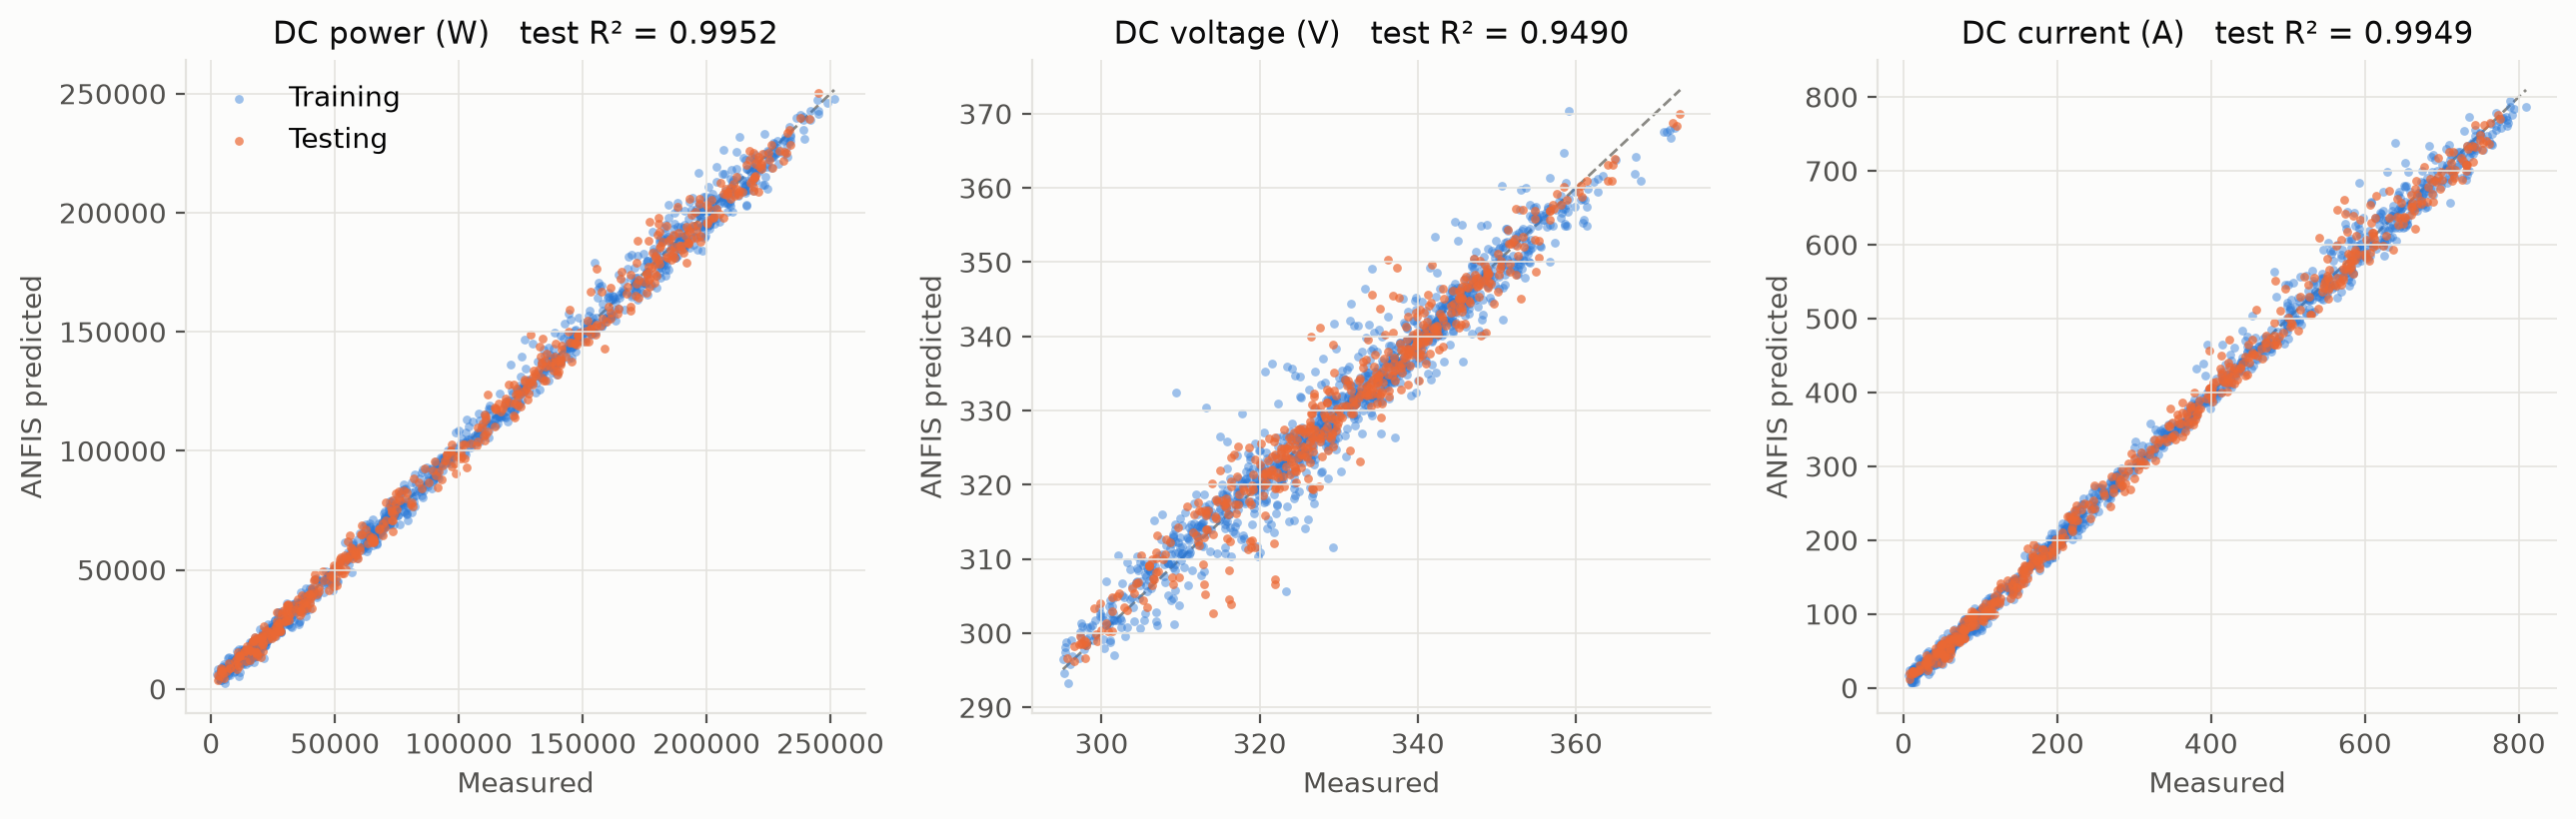
\includegraphics[width=0.92\linewidth]{fig1_anfis_pred_vs_measured.png}
\caption{ANFIS tahminleri ile ölçülen değerler (mavi: eğitim, turuncu: test). Kesikli çizgi mükemmel tahmini ($y=x$) gösterir.}
\label{fig:pred}
\end{figure}

Tablo~\ref{tab:t5} ve Şekil~\ref{fig:cmp}, güç tahmininde beş modelin karşılaştırmasını vermektedir. \textbf{Makalenin ana bulgusu yeniden üretilmiştir}: ANFIS en düşük test RMSE ve MAE değerine sahiptir. Bu sıralamanın tek bir bölmeye özgü olmadığını sınamak için deney 10 farklı rastgele bölmede tekrarlanmış; ANFIS 10 bölmenin 10'unda birinci olmuştur (ortalama RMSE: ANFIS 4878~W, rastgele orman 5601~W, SVM 5651~W). Karar ağacının eğitim hatası sıfır, test hatası ise yüksektir; bu, makalede de belirtilen aşırı öğrenmenin açık bir göstergesidir. Normalize hata açısından bizim tüm modellerimiz makaledekilerden yaklaşık 2–3 kat daha düşük hata vermektedir. Olası nedenler Bölüm~\ref{sec:disc}'de tartışılmıştır.

\begin{table}[H]
\centering\small
\caption{DC güç tahmininde model karşılaştırması (makale Tablo~5'in tekrarı). RMSE ve MAE watt cinsindendir.}
\label{tab:t5}
\begin{tabular}{@{}lrrrrrrc@{}}
\toprule
& \multicolumn{3}{c}{Bu çalışma — eğitim} & \multicolumn{3}{c}{Bu çalışma — test} & Makale test \\
\cmidrule(lr){2-4}\cmidrule(lr){5-7}\cmidrule(l){8-8}
Model & RMSE & MAE & $R^2$ & RMSE & MAE & $R^2$ & nRMSE / $R^2$ \\
\midrule
Doğrusal regresyon & 7400 & 5922 & 0,9894 & 7369 & 5997 & 0,9888 & \%14,7 / 0,938 \\
Karar ağacı & 0 & 0 & 1,0000 & 6861 & 5083 & 0,9902 & \%15,0 / 0,936 \\
SVM & 5295 & 4225 & 0,9945 & 5316 & 4233 & 0,9941 & \%14,8 / 0,937 \\
Rastgele orman & 2156 & 1584 & 0,9991 & 5183 & 3885 & 0,9944 & \%15,8 / 0,929 \\
\textbf{ANFIS} & 4606 & 3414 & 0,9959 & \textbf{4815} & \textbf{3626} & \textbf{0,9952} & \%12,2 / 0,996 \\
\bottomrule
\end{tabular}
\end{table}

\begin{figure}[H]
\centering
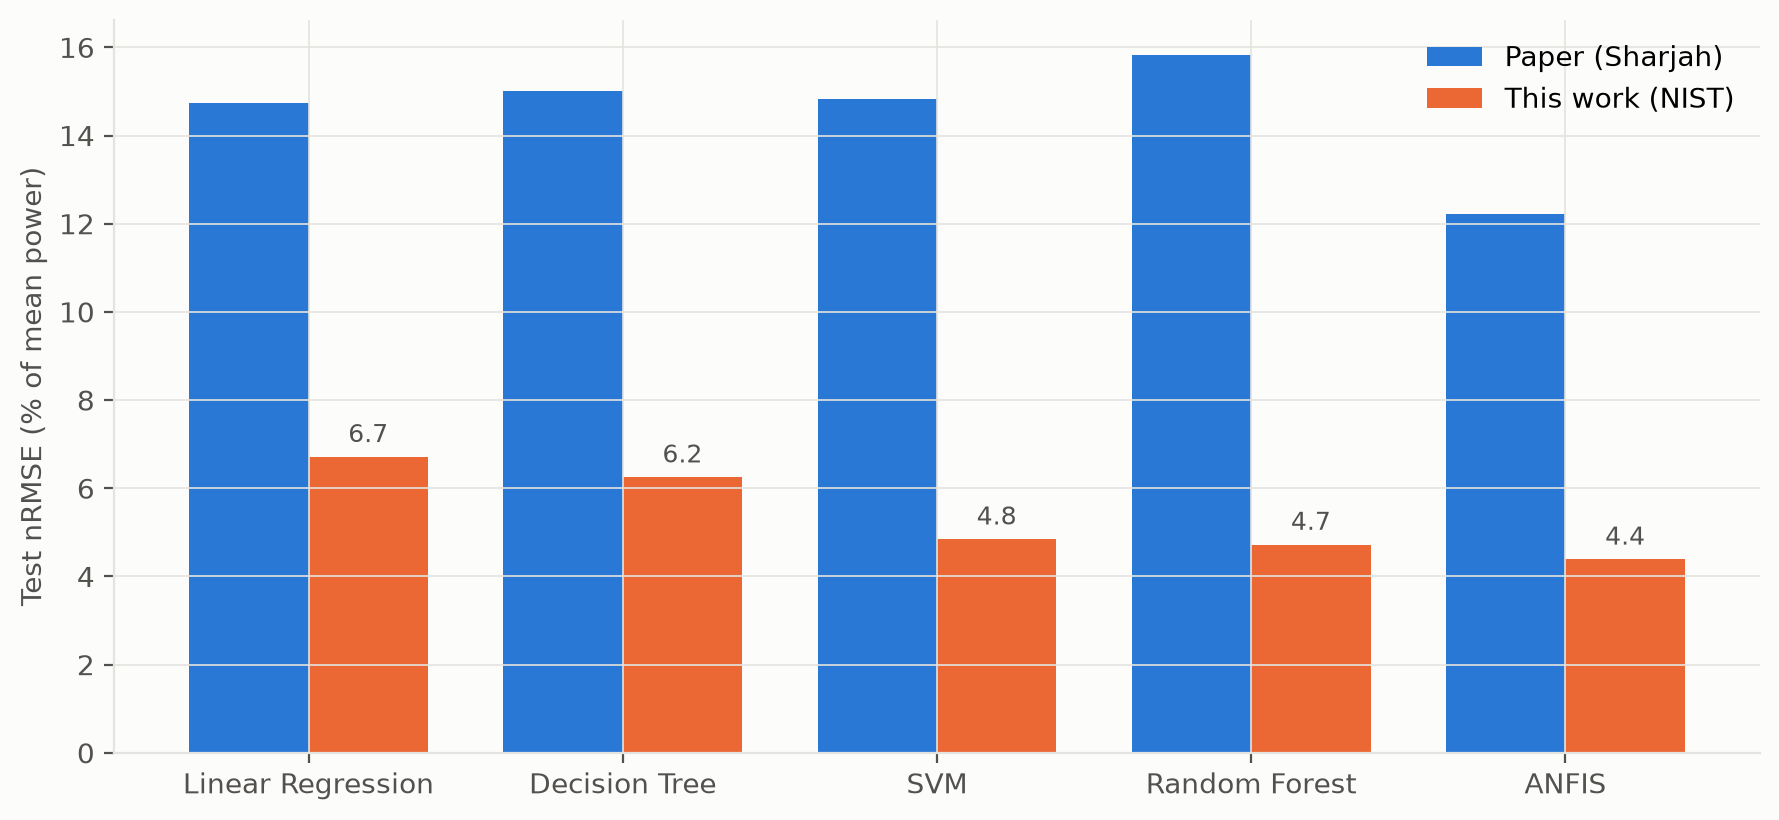
\includegraphics[width=0.68\linewidth]{fig5_model_comparison.png}
\caption{Test nRMSE: makale (Sharjah) ve bu çalışma (NIST). Sıralama korunmuş, ANFIS iki veri setinde de en iyi modeldir.}
\label{fig:cmp}
\end{figure}

\subsection{Öğrenilmiş kurallar}
Şekil~\ref{fig:mf} güç modelinin öğrenilmiş üyelik fonksiyonlarını, Tablo~\ref{tab:rules} ise kuralları orijinal birimlerde göstermektedir. Kurallar fiziksel olarak yorumlanabilir:
\begin{itemize}
\item Dört kuralın hepsinde ışınım katsayısı pozitiftir: her W/m² için 180–290~W. Bu, $\approx$250~kW'lık bir dizinin 1000~W/m²'de üreteceği güçle tutarlıdır.
\item “Sıcak panel” kuralında (K2, modül $\approx$61~°C) modül sıcaklığı katsayısı negatiftir (−3,5~kW/°C). Yani panel ısındıkça güç düşer; bu, makaledeki Denklem~13'teki negatif sıcaklık katsayısının veriden öğrenilmiş karşılığıdır \cite{paudyal2021}.
\item K4, serin sabah koşullarını temsil eder (ortam $\approx$16~°C, modül $\approx$8~°C).
\end{itemize}

\begin{figure}[H]
\centering
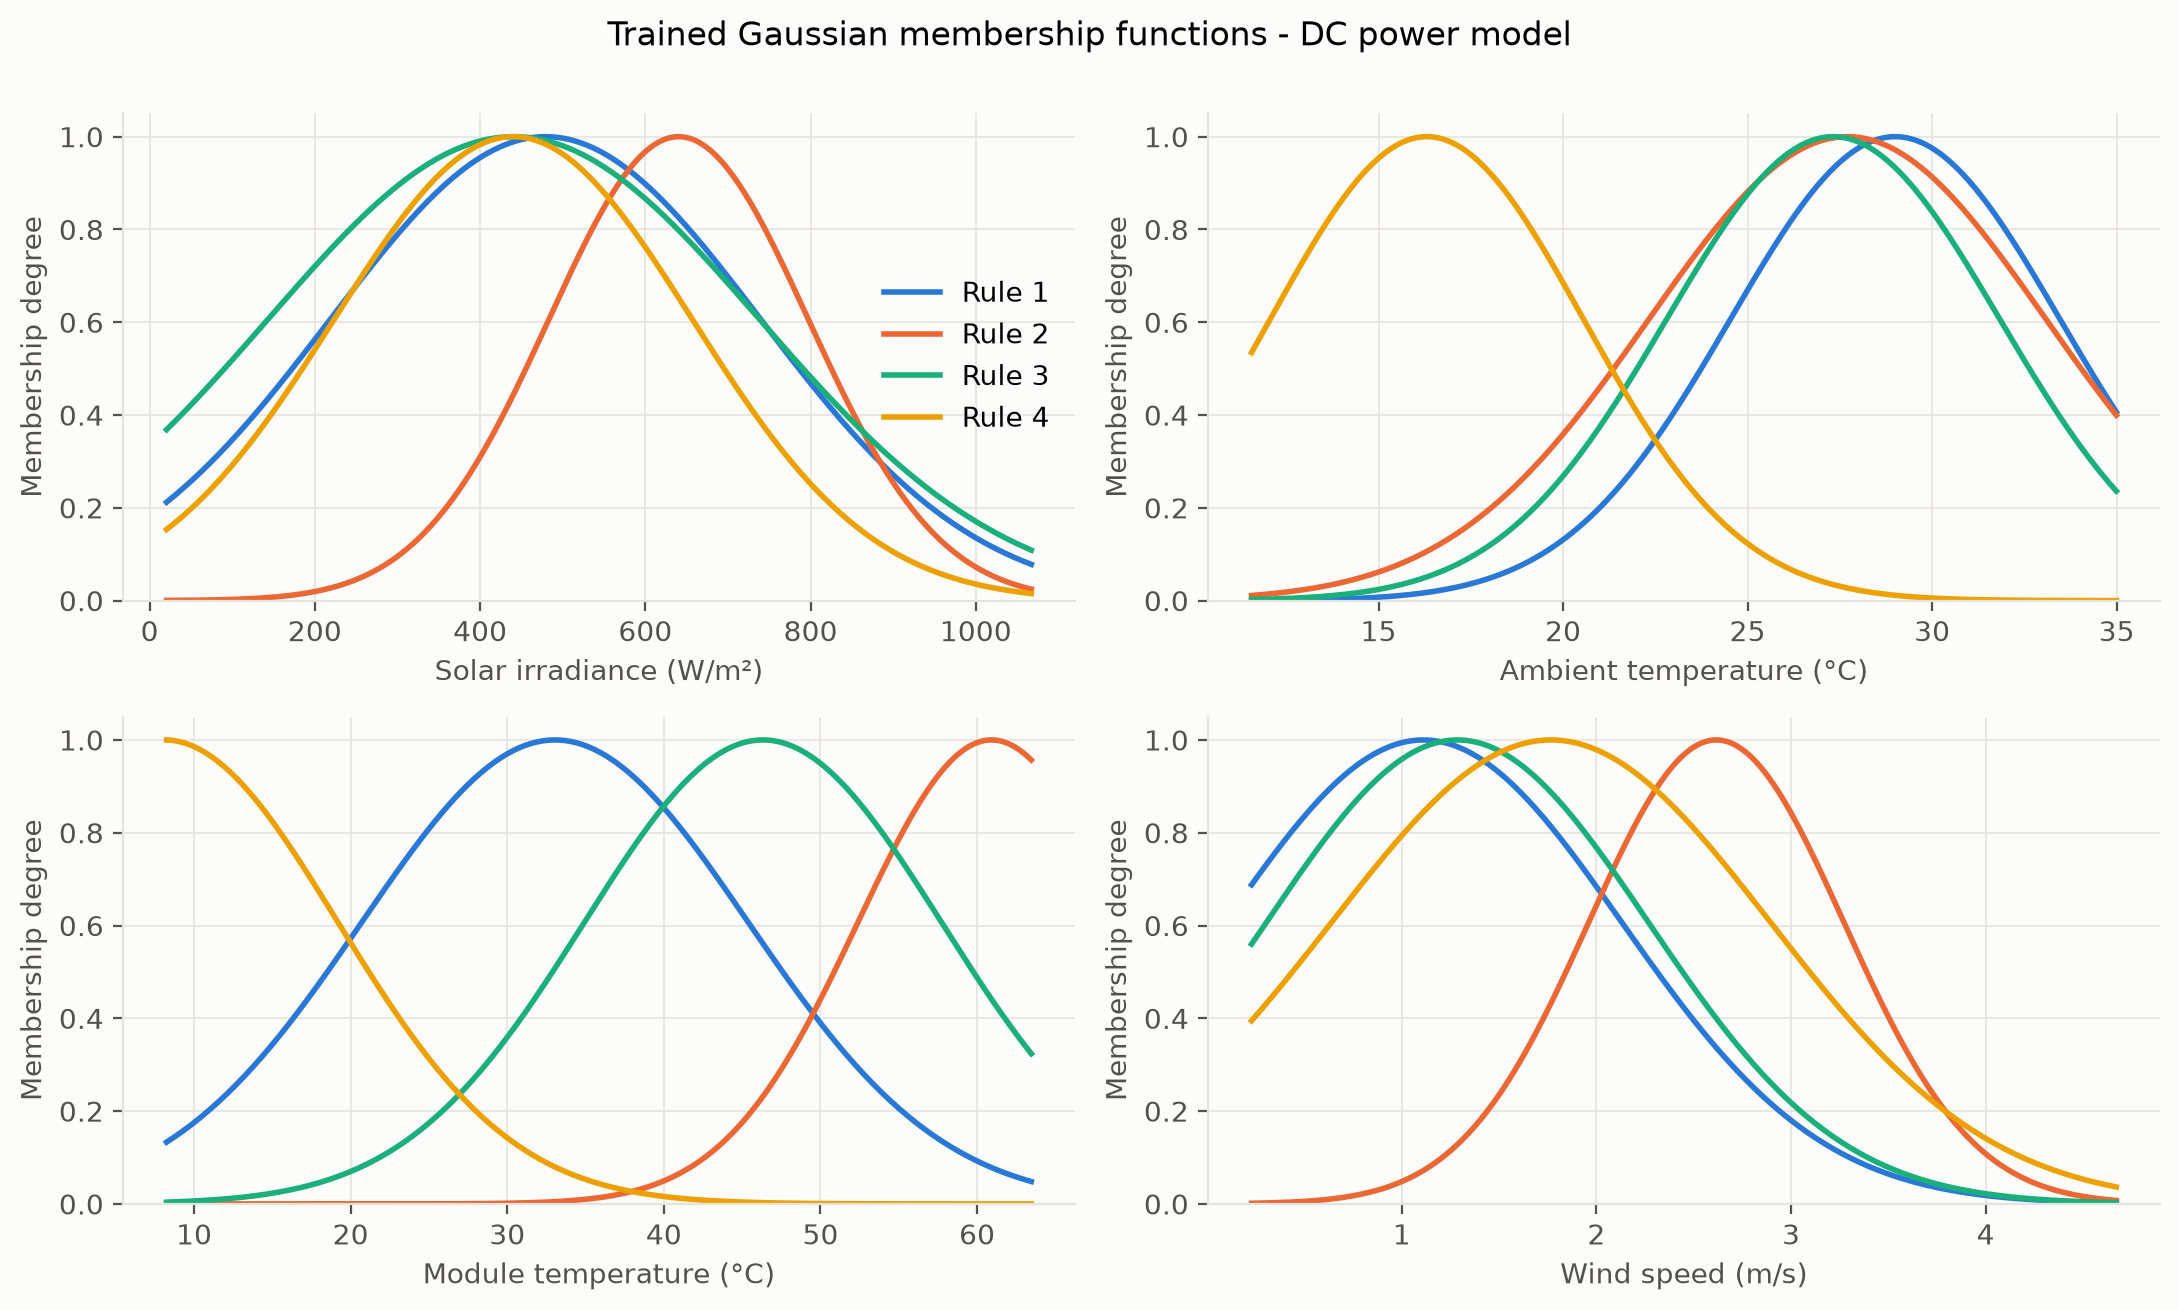
\includegraphics[width=0.66\linewidth]{fig3_mf_power.png}
\caption{DC güç modeli için eğitim sonrası Gauss üyelik fonksiyonları (her renk bir kural).}
\label{fig:mf}
\end{figure}

\begin{table}[H]
\centering\small
\caption{DC güç modelinin öğrenilmiş kuralları. Öncüller: Gauss merkezi (genişlik $\sigma$). Sonuç: $f_j$ katsayıları (W / birim).}
\label{tab:rules}
\begin{tabular}{@{}lllllrr@{}}
\toprule
Kural & Işınım (W/m²) & $T_\text{ortam}$ (°C) & $T_\text{modül}$ (°C) & Rüzgâr (m/s) & $\partial f/\partial G$ & $\partial f/\partial T_\text{modül}$ \\
\midrule
K1 ılık, orta ışınım & 479 (260) & 29,0 (4,5) & 33,0 (12,3) & 1,1 (1,0) & 180 & +4493 \\
K2 sıcak panel, yüksek ışınım & 640 (157) & 27,7 (5,4) & 60,9 (8,5) & 2,6 (0,7) & 270 & −3504 \\
K3 orta sıcaklık & 441 (297) & 27,3 (4,5) & 46,3 (11,4) & 1,3 (1,0) & 289 & −1429 \\
K4 serin sabah & 440 (217) & 16,3 (4,2) & 8,1 (11,1) & 1,8 (1,1) & 241 & +1269 \\
\bottomrule
\end{tabular}
\end{table}

\subsection{E1 — Kural tabanı karmaşıklığı}
Şekil~\ref{fig:rules} ve Tablo~\ref{tab:e1} sonuçları özetlemektedir:
\begin{itemize}
\item Tek kurallı ANFIS doğrusal regresyona eşdeğerdir (güç: \%6,75). Bu, uygulamanın doğruluğu için ayrıca bir sağlamadır.
\item 2–6 kural, üç çıktı için de en düşük hatayı vermektedir. Makalenin seçtiği 4 kural bu aralıktadır.
\item 8 kuralın üzerinde eğitim hatası düşmeye devam ederken test hatası ve bölmeler arası değişkenlik artmaktadır (güç, 11 kural: \%7,96 ± 3,64). Bu, aşırı öğrenmenin başladığını gösterir.
\item 81 kurallı grid partition, $\approx$1060 eğitim örneği için 1053 parametreye sahiptir ve çökmektedir (güç \%26,4, akım \%37,8).
\end{itemize}

\begin{figure}[H]
\centering
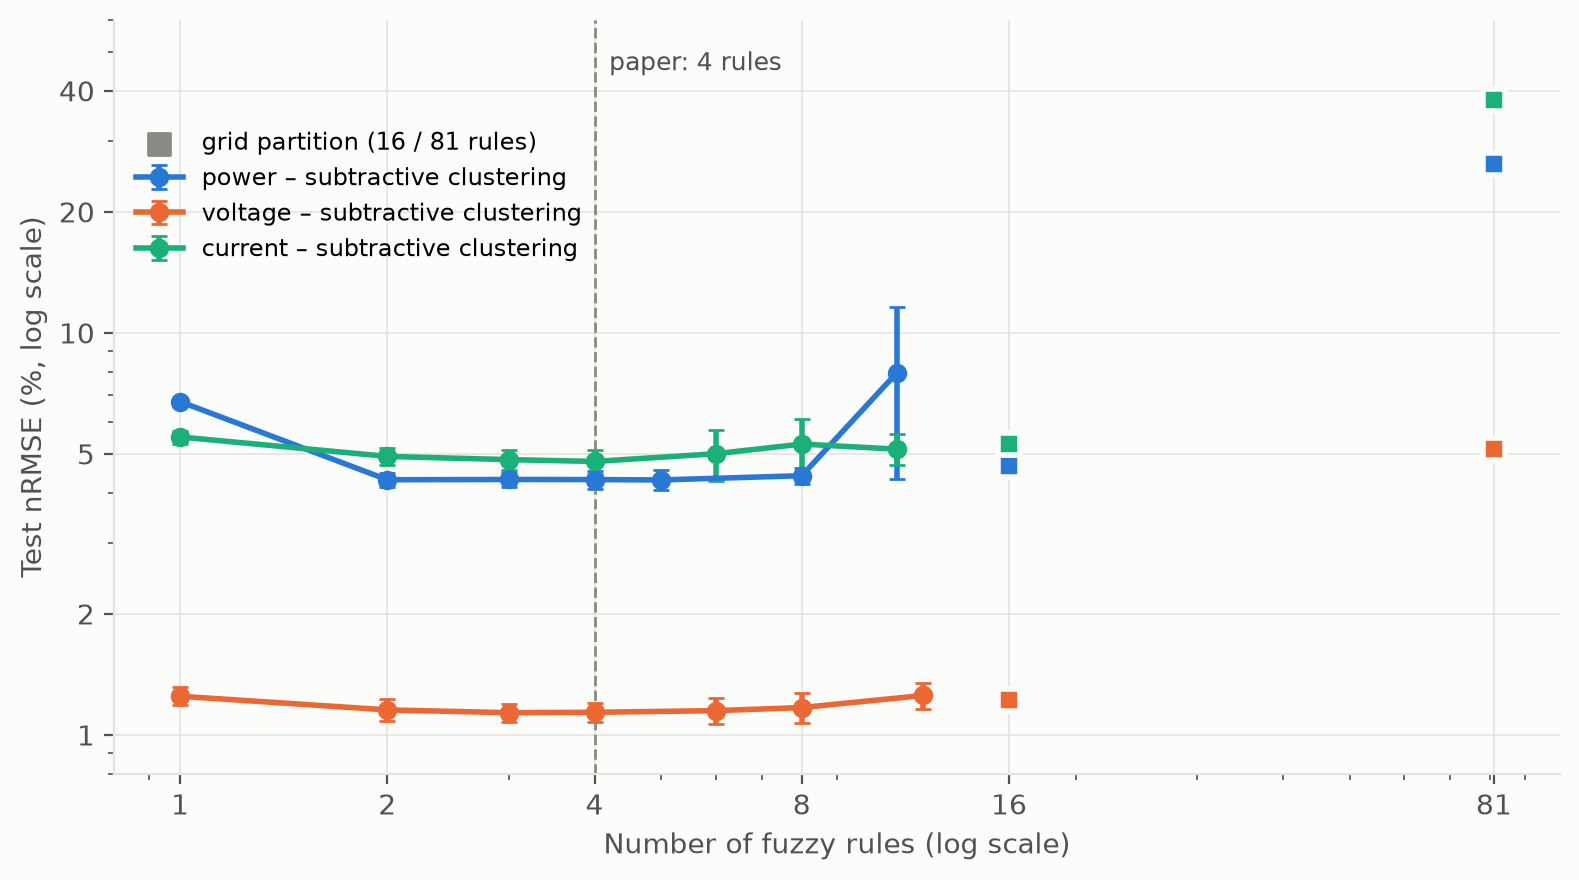
\includegraphics[width=0.66\linewidth]{fig6_rule_base_complexity.png}
\caption{Kural sayısına göre test nRMSE (5 bölme ortalaması ± std). Daireler subtractive clustering, kareler grid partition. Her iki eksen logaritmiktir.}
\label{fig:rules}
\end{figure}

\begin{table}[H]
\centering\small
\caption{E1: DC güç için kural tabanı karmaşıklığı (5 bölme ortalaması).}
\label{tab:e1}
\begin{tabular}{@{}lrrrr@{}}
\toprule
Kural tabanı & Kural & Parametre & Eğitim nRMSE (\%) & Test nRMSE (\%) \\
\midrule
SC, 1 kural & 1 & 13 & 6,71 & 6,75 ± 0,04 \\
SC, 2 kural & 2 & 26 & 4,35 & 4,31 ± 0,17 \\
\textbf{SC, 4 kural (makale)} & 4 & 52 & 4,18 & \textbf{4,32 ± 0,22} \\
SC, 8 kural & 8 & 104 & 3,97 & 4,41 ± 0,20 \\
SC, 11 kural & 11 & 143 & 3,77 & 7,96 ± 3,64 \\
Grid, 2 MF/girdi & 16 & 208 & 3,92 & 4,68 ± 0,42 \\
Grid, 3 MF/girdi & 81 & 1053 & 2,10 & 26,37 ± 8,00 \\
\bottomrule
\end{tabular}
\end{table}

\subsection{E2 — Rastgele ve kronolojik bölme}
Kronolojik bölmede (Şekil~\ref{fig:chrono}) ANFIS'in hatası neredeyse değişmemektedir (\%4,39 → \%4,46). Diğer modeller ise belirgin biçimde kötüleşmektedir: SVM \%4,84 → \%7,66, rastgele orman \%4,72 → \%5,85, karar ağacı \%6,25 → \%7,59. ANFIS ile en yakın rakibi arasındaki fark kronolojik bölmede büyümektedir. Dolayısıyla makalenin “ANFIS daha iyi genelleştirir” iddiası, daha gerçekçi bir protokolde daha da güçlü biçimde desteklenmektedir.

\begin{figure}[H]
\centering
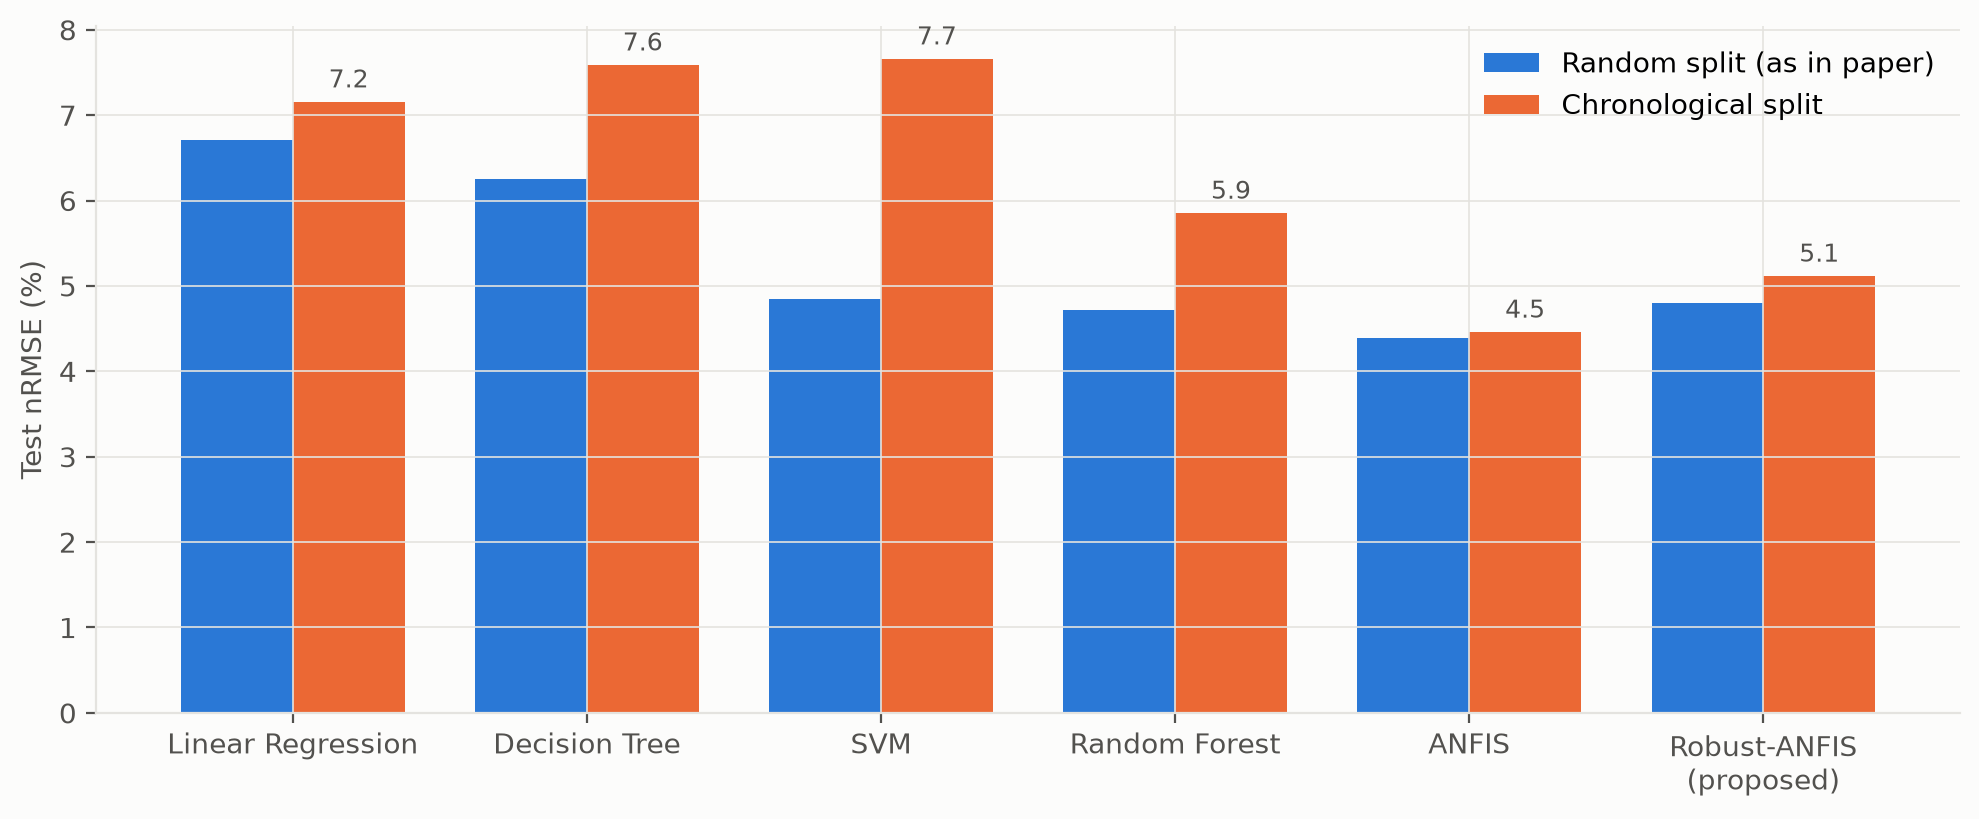
\includegraphics[width=0.72\linewidth]{fig7_random_vs_chronological.png}
\caption{Rastgele (makaledeki) ve kronolojik bölmede DC güç test nRMSE değerleri.}
\label{fig:chrono}
\end{figure}

\subsection{E3 ve E4 — Sensör gürültüsü ve Robust-ANFIS}
Şekil~\ref{fig:noise} ve Tablo~\ref{tab:noise}, girdi gürültüsü arttıkça modellerin davranışını göstermektedir. \textbf{Temiz veride en iyi olan ANFIS, gürültüye en duyarlı modeldir}: sensör hassasiyeti düzeyinde (düzey~1) hatası \%4,32'den \%8,06'ya çıkar ve SVM (\%7,39) ile rastgele ormanın (\%7,19) gerisine düşer. İki kat gürültüde (\%14,68) doğrusal regresyondan bile kötüdür. Önerilen Robust-ANFIS bu düzeylerde sırasıyla \%6,74 ve \%10,49 hata verir ve gerçekçi gürültüde tüm modeller arasında en düşük hataya ulaşır. Aynı gürültüyle eğitilmiş SVM çok yakındır (\%6,83). Karar ağacı ve rastgele orman gürültü enjeksiyonundan pek yarar görmez; karar ağacı temiz veride belirgin biçimde kötüleşir (\%6,46 → \%8,21).

\begin{figure}[H]
\centering
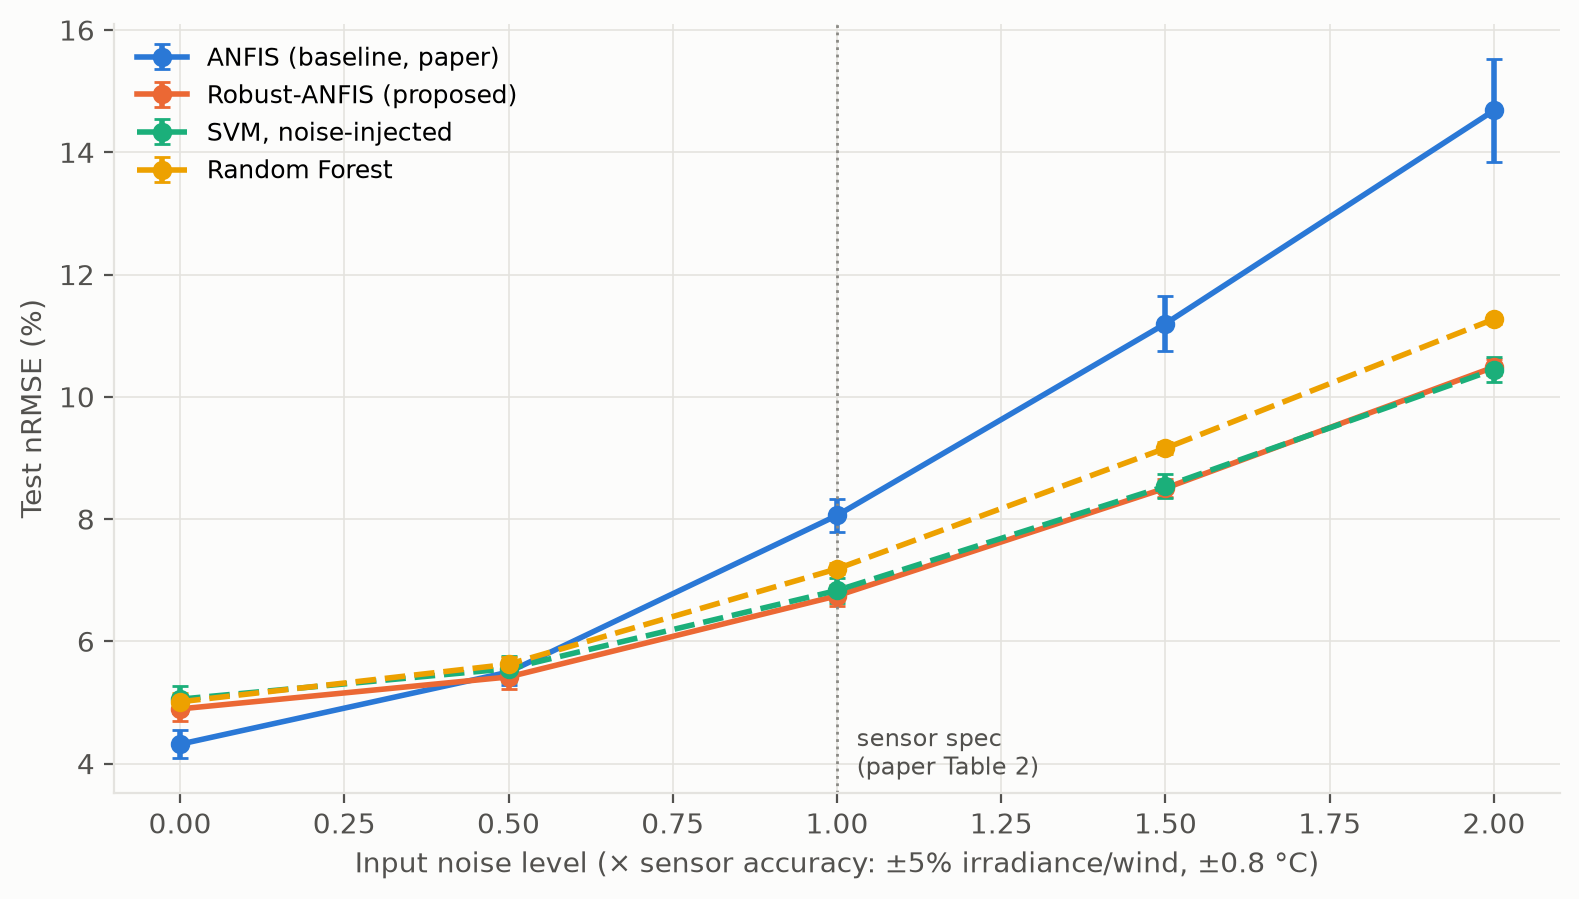
\includegraphics[width=0.66\linewidth]{fig8_noise_robustness.png}
\caption{Girdi gürültüsü düzeyine göre DC güç test nRMSE (5 bölme × 10 gürültü örneği; hata çubukları bölmeler arası std). Düzey~1, makalenin Tablo~2'sindeki sensör hassasiyetidir.}
\label{fig:noise}
\end{figure}

\begin{table}[H]
\centering\small
\caption{E3: Gürültü düzeyine göre DC güç test nRMSE (\%). “Temiz”: temiz veriyle eğitim; “GE”: gürültü enjeksiyonlu eğitim.}
\label{tab:noise}
\begin{tabular}{@{}llrrrrr@{}}
\toprule
Model & Eğitim & 0 & 0,5 & 1 & 1,5 & 2 \\
\midrule
ANFIS (makale) & Temiz & \textbf{4,32} & 5,50 & 8,06 & 11,20 & 14,68 \\
\textbf{Robust-ANFIS (önerilen)} & GE & 4,89 & \textbf{5,42} & \textbf{6,74} & \textbf{8,51} & 10,49 \\
SVM & Temiz & 5,01 & 5,71 & 7,39 & 9,51 & 11,78 \\
SVM & GE & 5,05 & 5,55 & 6,83 & 8,54 & \textbf{10,44} \\
Rastgele orman & Temiz & 5,01 & 5,62 & 7,19 & 9,16 & 11,27 \\
Rastgele orman & GE & 5,50 & 6,02 & 7,25 & 8,90 & 10,84 \\
Karar ağacı & Temiz & 6,46 & 7,06 & 8,36 & 10,24 & 12,19 \\
Doğrusal regresyon & Temiz & 6,75 & 7,35 & 8,83 & 10,85 & 13,15 \\
\bottomrule
\end{tabular}
\end{table}

Tablo~\ref{tab:e4}, yönergedeki formatta baseline ve önerilen yöntemi karşılaştırmaktadır. Gerilim ve akım modellerinde de aynı eğilim görülmüştür. Sensör düzeyindeki gürültüde akım hatası \%8,81'den \%7,30'a, gerilim hatası \%1,25'ten \%1,20'ye inmiş; temiz veride ise sırasıyla \%4,79 → \%5,43 ve \%1,14 → \%1,16 olarak hafifçe artmıştır.

\begin{table}[H]
\centering\small
\caption{E4: Baseline ANFIS ile Robust-ANFIS karşılaştırması, DC güç (5 bölme ortalaması). Süreler makineye göre değişebilir.}
\label{tab:e4}
\begin{tabular}{@{}lrrr@{}}
\toprule
Performans ölçütü & Baseline ANFIS & Robust-ANFIS & Değişim \\
\midrule
$R^2$ (temiz test) & 0,9954 & 0,9941 & $-$\%0,1 \\
RMSE (W, temiz test) & 4811 & 5454 & +\%13,4 \\
nRMSE (\%, temiz test) & 4,32 & 4,89 & +\%13,4 \\
nRMSE (\%, sensör düzeyi gürültü) & 8,06 & \textbf{6,74} & \textbf{$-$\%16,3} \\
nRMSE (\%, 2× sensör gürültüsü) & 14,68 & \textbf{10,49} & \textbf{$-$\%28,6} \\
Eğitim süresi (s) & 0,68 & 0,92 & +\%35 \\
Çıkarım süresi (µs/örnek) & 0,25 & 0,27 & $\approx$ aynı \\
Parametre sayısı & 52 & 52 & 0 \\
\bottomrule
\end{tabular}
\end{table}

\subsection{E5 — Dayanıklılığın mekanizması}
Hangi girdideki gürültünün etkili olduğunu ayırt etmek için sensör düzeyindeki gürültü her seferinde yalnızca tek bir girdiye eklenmiştir (Tablo~\ref{tab:e5}). Ayrıca iki ANFIS modelinin her girdiye ortalama duyarlılığı sayısal türevle ölçülmüştür. Yorum Bölüm~\ref{sec:disc}'dedir.

\begin{table}[H]
\centering\small
\caption{E5: Sensör düzeyindeki gürültü yalnızca tek bir girdiye eklendiğinde DC güç test nRMSE (\%) ve ANFIS modellerinin ortalama girdi duyarlılığı (girdinin 1 std'si başına kW). 5 bölme ortalaması.}
\label{tab:e5}
\begin{tabular}{@{}lrrrr@{}}
\toprule
& Işınım & $T_\text{ortam}$ & $T_\text{modül}$ & Rüzgâr \\
\midrule
\multicolumn{5}{@{}l}{\emph{Yalnızca bu girdi gürültülüyken nRMSE (\%)}}\\
ANFIS (baseline) & 7,69 & 4,49 & 4,55 & 4,35 \\
Robust-ANFIS & \textbf{6,66} & 4,95 & 4,92 & 4,90 \\
SVM & 7,23 & 5,10 & 5,10 & 5,07 \\
Rastgele orman & 7,15 & 5,02 & 5,02 & 5,01 \\
\midrule
\multicolumn{5}{@{}l}{\emph{Ortalama duyarlılık $\overline{\partial P/\partial x}$ (kW / 1 std); parantez içinde ortalama mutlak değer}}\\
ANFIS (baseline) & 77,2 & 2,5 (5,6) & $-$8,0 (17,1) & $-$0,6 (1,7) \\
Robust-ANFIS & 66,5 & $-$3,8 (4,0) & 5,4 (6,9) & 1,9 (2,0) \\
\bottomrule
\end{tabular}
\end{table}

% =====================================================================
\section{Discussion — Tartışma}
\label{sec:disc}

\textbf{Neden makaleden daha düşük hata?} Normalize hatalarımız tüm modellerde makaledekinin yaklaşık üçte biridir. Bunun en olası üç nedeni vardır. (i) Veri miktarı: makalede 601, bizde 1555 örnek vardır. (ii) Ölçek: 250~kW'lık bir dizide çok sayıda panelin ortalaması alındığı için tekil panel kaynaklı oynamalar sönümlenir, oysa 9 panelli bir sistemde bu etki büyüktür. (iii) Saatlik ortalama: bir saatlik ortalama ani bulut geçişlerini yumuşatır. Makale ise örnekleme aralığını tutarlı biçimde belirtmemektedir. Ayrıca makalenin Tablo~5'teki ANFIS $R^2$ değeri, aynı tablodaki RMSE ile tutarsızdır (Bölüm~4.3). Bu nedenle mutlak değerler yerine modeller arası \emph{sıralama} karşılaştırılmalıdır. Sıralama iki veri setinde de aynıdır.

\textbf{Neden ANFIS kronolojik bölmede daha iyi?} ANFIS'in her kuralı yerel bir doğrusal model olduğundan, model ışınım–güç ilişkisini fiziksel olarak anlamlı ve düzgün (smooth) bir fonksiyonla yakalar. Karar ağacı ve rastgele orman ise girdi uzayını basamaklara böler ve eğitimde az görülen bölgelerde (ör. Ağustos sonu–Eylül'ün daha serin günleri) zayıf kalır. SVM'nin kronolojik bölmedeki büyük kaybı (\%4,8 → \%7,7) için olası bir açıklama, varsayılan RBF çekirdek genişliğinin dağılım kaymasına duyarlı olmasıdır; bu tahmin ayrıca test edilmemiştir.

\textbf{Neden ANFIS gürültüye duyarlı ve Robust-ANFIS neden daha dayanıklı?} Başlangıçtaki tahminimiz, Tablo~\ref{tab:rules}'deki büyük ve zıt işaretli sıcaklık katsayılarının sorumlu olduğuydu. E5 deneyi bu tahmini \emph{çürütmüştür}. Gürültü yalnızca sıcaklık veya rüzgâra eklendiğinde ANFIS'in hatası neredeyse değişmemektedir (\%4,3 → \%4,5). Bozulmanın neredeyse tamamı ışınım gürültüsünden gelmektedir (Tablo~\ref{tab:e5}). Baseline ANFIS gücü büyük ölçüde ışınımın doğrusal bir fonksiyonu olarak öğrenmiştir: ışınımın 1 standart sapmalık değişimi ortalama 77,2~kW güç değişimi yaratır. Bu nedenle ışınımdaki \%5'lik ölçüm hatası doğrudan çıktıya taşınır. Gürültü enjeksiyonu, beklenen kayıpta gürültülü girdiye göre türevi cezalandıran bir düzenlileştirme etkisi yaratır~\cite{bishop1995}. Nitekim Robust-ANFIS'in ışınım duyarlılığı \%14 azalmış (66,5~kW), modül sıcaklığına yanıtı ise daha düzgün hâle gelmiştir (ortalama mutlak duyarlılık 17,1 → 6,9~kW). Işınım ile modül sıcaklığı güçlü biçimde ilişkili olduğundan ($r=0{,}88$), model ışınım ölçümü hatalı olduğunda modül sıcaklığını kısmen yedek bir sinyal olarak kullanmayı öğrenmektedir. Robust-ANFIS'te modül sıcaklığının ortalama etkisinin pozitif çıkması bu nedenledir. Bu etki, fiziksel sıcaklık kaybını değil, ışınımla olan ilişkiyi yansıtır. Kazancın temiz veride küçük bir kayıpla gelmesi beklenen yanlılık–varyans dengesidir.

\textbf{Pratik sonuç.} Hangi modelin kullanılacağı sahadaki sensör kalitesine bağlıdır. Kalibre, yüksek hassasiyetli sensörlerde baseline ANFIS; sensör hassasiyetinin ±\%5 düzeyinde olduğu tipik saha kurulumlarında ise Robust-ANFIS daha uygundur. Önerilen yöntem model yapısını değiştirmediği için yorumlanabilirlik korunur ve dağıtım maliyeti artmaz.

% =====================================================================
\section{Limitations — Sınırlılıklar}
\begin{itemize}
\item \textbf{Farklı saha.} Ilıman iklimdeki (Maryland, ABD) ve $\approx$90 kat büyük bir sistemle çalışılmıştır. Sharjah'ın sıcak ve tozlu koşulları, özellikle modül sıcaklığı etkileri, birebir temsil edilmemektedir.
\item \textbf{Eksik ayrıntılar.} Makale yarıçap, epok, bölme yöntemi ve hiperparametre bildirmediğinden bu değerler tarafımızca seçilmiştir. Farklı seçimler mutlak sayıları değiştirebilir.
\item \textbf{Basitleştirilmiş gürültü modeli.} Gürültü bağımsız Gauss olarak modellenmiştir. Gerçek sensör hataları sistematik sapma (bias), kirlenme veya zamanla kayma (drift) içerebilir.
\item \textbf{Tek mevsim.} Yalnızca tek bir yılın yaz dönemi kullanılmıştır. Kış ve geçiş mevsimlerinde performans test edilmemiştir.
\item \textbf{Hiperparametre ayarı yok.} Karşılaştırma modelleri varsayılan ayarlarla kullanılmıştır. Ayarlanmış bir SVM veya rastgele orman farkı kapatabilir.
\item \textbf{Kestirim, tahmin değil.} Makaledeki gibi model eşzamanlı ölçümlerden kestirim yapar. Hava tahmini girdileriyle ileriye dönük tahmin ek belirsizlik getirecektir.
\end{itemize}

% =====================================================================
\section{Conclusion — Sonuç}
Referans makaledeki ANFIS yöntemi açık bir veri setinde, sıfırdan yazılmış bir uygulama ile yeniden gerçekleştirilmiş ve makalenin ana bulgusu doğrulanmıştır: ANFIS, dört çevresel girdiden DC güç, gerilim ve akımı $R^2\geq0{,}949$ ile kestirmekte ve güç tahmininde dört klasik modelden daha iyi sonuç vermektedir. Bu üstünlüğün kaynağı, girdilerdeki gürültüye değil, modelin ışınım–güç ilişkisini doğrudan öğrenmesidir; aynı özellik onu ışınım ölçüm hatasına karşı kırılgan da yapmaktadır. Genişletme deneyleri şunları göstermiştir: (1) subtractive clustering ile 2–6 kural yeterlidir, makalenin 4 kural seçimi isabetlidir ve grid partition 4 girdide hızla aşırı öğrenmeye gider; (2) ANFIS'in üstünlüğü kronolojik bölmede korunmakta, hatta büyümektedir; (3) ANFIS gerçekçi sensör gürültüsüne karşı en kırılgan modeldir. Önerilen Robust-ANFIS bu zayıflığı yapıyı değiştirmeden gidermiş, sensör düzeyindeki gürültüde hatayı \%16 azaltarak tüm modeller arasında en iyi sonuca ulaşmıştır.

Gelecek çalışmalar için şu yönler önerilmektedir: farklı mevsimlerde ve iklimlerde doğrulama; gürültü seviyesinin çapraz doğrulama ile seçilmesi; sistematik sensör hatalarının (bias, drift) modellenmesi; Tip-2 bulanık kümeler gibi belirsizliği doğrudan temsil eden yapıların Robust-ANFIS ile karşılaştırılması; hava tahmini girdileriyle gerçek ileriye dönük tahmin.

% =====================================================================
\section*{Generative AI Usage Disclosure — Üretken Yapay Zekâ Kullanım Beyanı}
Bu projede Anthropic'in Claude modeli yardımcı araç olarak kullanılmıştır. Kullanım alanları şunlardır: referans makale ve proje yönergesinin özetlenmesi; açık veri seti seçeneklerinin araştırılması; veri hazırlama, ANFIS ve deney kodlarının taslaklarının yazılması; deney tasarımı için öneriler; şekillerin üretilmesi ve bu raporun taslağının hazırlanması. İlgili çalışmalar bölümündeki kaynaklar referans makalenin kaynakçasından alınmış ve künyeleri oradan kontrol edilmiştir. Kodun tamamı öğrenci tarafından kendi bilgisayarında çalıştırılmış ve rapordaki sayıların üretilen tablolarla birebir aynı olduğu doğrulanmıştır. ANFIS gradyanları sonlu farklarla ayrıca sınanmıştır. Raporun ve kodun içeriğinden öğrenci sorumludur.

% =====================================================================
\begin{thebibliography}{99}
\small

\bibitem{salameh2025}
T.~Salameh, M.~M. Farag, A.-K. Hamid, and M.~Hussein, ``Adaptive neuro-fuzzy inference system for accurate power forecasting for on-grid photovoltaic systems: A case study in Sharjah, UAE,'' \emph{Energy Convers. Manage.: X}, vol.~26, Art.~no.~100958, 2025, doi: 10.1016/j.ecmx.2025.100958.

\bibitem{gaboitaolelwe2023}
J.~Gaboitaolelwe, A.~M. Zungeru, A.~Yahya, C.~K. Lebekwe, D.~N. Vinod, and A.~O. Salau, ``Machine learning based solar photovoltaic power forecasting: A review and comparison,'' \emph{IEEE Access}, vol.~11, pp.~40820--40845, 2023, doi: 10.1109/ACCESS.2023.3270041.

\bibitem{jang1993}
J.-S.~R. Jang, ``ANFIS: Adaptive-network-based fuzzy inference system,'' \emph{IEEE Trans. Syst., Man, Cybern.}, vol.~23, no.~3, pp.~665--685, 1993, doi: 10.1109/21.256541.

\bibitem{xiang2024}
X.~Xiang, X.~Li, Y.~Zhang, and J.~Hu, ``A short-term forecasting method for photovoltaic power generation based on the TCN-ECANet-GRU hybrid model,'' \emph{Sci. Rep.}, vol.~14, Art.~no.~6744, 2024, doi: 10.1038/s41598-024-56751-6.

\bibitem{fan2024}
Y.~Fan, Z.~Ma, W.~Tang, J.~Liang, and P.~Xu, ``Using Crested Porcupine Optimizer algorithm and CNN-LSTM-attention model combined with deep learning methods to enhance short-term power forecasting in PV generation,'' \emph{Energies}, vol.~17, Art.~no.~3435, 2024, doi: 10.3390/en17143435.

\bibitem{ibrahim2024}
M.~S. Ibrahim, S.~M. Gharghory, and H.~A. Kamal, ``A hybrid model of CNN and LSTM autoencoder-based short-term PV power generation forecasting,'' \emph{Electr. Eng.}, vol.~106, pp.~4239--4255, 2024, doi: 10.1007/s00202-023-02220-8.

\bibitem{aitmansour2024}
A.~Ait~Mansour, A.~Tilioua, and M.~Touzani, ``Bi-LSTM, GRU and 1D-CNN models for short-term photovoltaic panel efficiency forecasting case amorphous silicon grid-connected PV system,'' \emph{Results Eng.}, vol.~21, Art.~no.~101886, 2024, doi: 10.1016/j.rineng.2024.101886.

\bibitem{bashir2024}
S.~B. Bashir, M.~M. Farag, A.~K. Hamid, A.~A. Adam, A.~G. Abo-Khalil, and R.~Bansal, ``A novel hybrid CNN-XGBoost model for photovoltaic system power forecasting,'' in \emph{Proc. 6th Int. Youth Conf. Radio Electron., Electr. Power Eng. (REEPE)}, 2024, pp.~1--6, doi: 10.1109/REEPE60449.2024.10479878.

\bibitem{guerra2024}
M.~I.~S. Guerra, F.~M.~U. de~Araújo, J.~T. de~Carvalho~Neto, and R.~G. Vieira, ``Survey on adaptative neural fuzzy inference system (ANFIS) architecture applied to photovoltaic systems,'' \emph{Energy Syst.}, vol.~15, pp.~505--541, 2024, doi: 10.1007/s12667-022-00513-8.

\bibitem{perveen2019}
G.~Perveen, M.~Rizwan, and N.~Goel, ``An ANFIS-based model for solar energy forecasting and its smart grid application,'' \emph{Eng. Rep.}, vol.~1, Art.~no.~e12070, 2019, doi: 10.1002/eng2.12070.

\bibitem{bouachrine2023}
B.~Bouachrine, M.~Oubella, K.~Dahmane, and M.~Ajaamoum, ``ANFIS model to calculate open circuit voltage and maximum power voltage to effectively emulate the electrical characteristics of four photovoltaic technologies,'' \emph{Appl. Sol. Energy}, vol.~59, pp.~779--790, 2023, doi: 10.3103/S0003701X22600771.

\bibitem{ramadan2022}
A.~Ramadan, S.~Kamel, I.~Hamdan, and A.~M. Agwa, ``A novel intelligent ANFIS for the dynamic model of photovoltaic systems,'' \emph{Mathematics}, vol.~10, Art.~no.~1286, 2022, doi: 10.3390/math10081286.

\bibitem{ren2024}
Z.~Ren and Y.~Zhou, ``On soft measurement modeling for predicting photovoltaic power with uncertainty based on the Takagi–Sugeno model,'' \emph{Meas. Sci. Technol.}, vol.~35, Art.~no.~115107, 2024, doi: 10.1088/1361-6501/ad6921.

\bibitem{massidda2024}
L.~Massidda, F.~Bettio, and M.~Marrocu, ``Probabilistic day-ahead prediction of PV generation. A comparative analysis of forecasting methodologies and of the factors influencing accuracy,'' \emph{Sol. Energy}, vol.~271, Art.~no.~112422, 2024, doi: 10.1016/j.solener.2024.112422.

\bibitem{bishop1995}
C.~M. Bishop, ``Training with noise is equivalent to Tikhonov regularization,'' \emph{Neural Comput.}, vol.~7, no.~1, pp.~108--116, 1995, doi: 10.1162/neco.1995.7.1.108.

\bibitem{zadeh1965}
L.~A. Zadeh, ``Fuzzy sets,'' \emph{Inf. Control}, vol.~8, no.~3, pp.~338--353, 1965, doi: 10.1016/S0019-9958(65)90241-X.

\bibitem{mamdani1975}
E.~H. Mamdani and S.~Assilian, ``An experiment in linguistic synthesis with a fuzzy logic controller,'' \emph{Int. J. Man-Mach. Stud.}, vol.~7, no.~1, pp.~1--13, 1975, doi: 10.1016/S0020-7373(75)80002-2.

\bibitem{takagi1985}
T.~Takagi and M.~Sugeno, ``Fuzzy identification of systems and its applications to modeling and control,'' \emph{IEEE Trans. Syst., Man, Cybern.}, vol.~SMC-15, no.~1, pp.~116--132, 1985, doi: 10.1109/TSMC.1985.6313399.

\bibitem{chiu1994}
S.~L. Chiu, ``Fuzzy model identification based on cluster estimation,'' \emph{J. Intell. Fuzzy Syst.}, vol.~2, no.~3, pp.~267--278, 1994.

\bibitem{nist}
National Institute of Standards and Technology, ``NIST campus photovoltaic (PV) arrays and weather station data sets,'' 2020. [Online]. Available: https://doi.org/10.18434/M3S67G

\bibitem{kingma2015}
D.~P. Kingma and J.~Ba, ``Adam: A method for stochastic optimization,'' in \emph{Proc. 3rd Int. Conf. Learn. Represent. (ICLR)}, San Diego, CA, USA, 2015.

\bibitem{pedregosa2011}
F.~Pedregosa \emph{et al.}, ``Scikit-learn: Machine learning in Python,'' \emph{J. Mach. Learn. Res.}, vol.~12, pp.~2825--2830, 2011.

\bibitem{paudyal2021}
B.~R. Paudyal and A.~G. Imenes, ``Investigation of temperature coefficients of PV modules through field measured data,'' \emph{Sol. Energy}, vol.~224, pp.~425--439, 2021, doi: 10.1016/j.solener.2021.06.013.

\end{thebibliography}

\end{document}
